\chapter{گرافلت کرنل گاوسی}\label{chap:gaussian-graphlet-kernel}
گرافلت‌ها انتخاب خوبی برای مقایسه دو گراف هستند. دلیل این انتخاب اولاً \خمیده{فرضیه بازسازی گراف}\پانوشت{\متن‌لاتین{graph reconstruction conjecture}}\جستار{Kelly_1957} است که بیان می‌کند هر گراف بطور یکتا توسط زیرگراف‌هایش مشخص می‌شود. بنابراین انتظار داریم اگر دو گراف شبیه هم باشند، گردایه‌ی زیرگراف‌های آن‌ها نیز مشابه باشد. ثانیاً به دلیل استفاده از تعداد زیرگراف‌های با اندازه ثابت، این مقایسه دچار مشکل رفت و برگشت و هالتینگ نمی‌شود.
در این فصل ابتدا نحوه شمارش گرافلت‌ها را شرح داده و سپس گرافلت کرنل گاوسی را معرفی می‌کنیم و به سنجش قدرت آن در جداسازی مدل‌های تصادفی گراف از یکدیگر، می‌پردازیم.

\section{گرافلت‌ها و شمارش آن‌ها}
گرافلت‌ها، زیرگراف‌های کوچک القایی بین سه تا پنج رأس از یک گراف بزرگتر هستند\جستار{Przulj_2004} که با برچسب $G1,\ldots,G29$ در شکل \ارجا{fig:graphlets} نمایش داده شده‌اند (معمولاً زیرگراف تک یالی $G0$ هم به این مجموعه اضافه می‌شود).  رئوس هر گرافلت به گروه‌های خودریختی\پانوشت{\متن‌لاتین{automorphism}} تقسیم می‌شوند که به آن‌ها اوربیت\پانوشت{\متن‌لاتین{orbit}} گفته می‌شود. دو رأس از یک گرافلت به یک اوربیت تعلق دارند اگر توسط یک تابع خودریختی به یکدیگر نگاشت شوند. در شکل \ارجا{fig:graphlets}، اوربیت‌ها با اعداد صفر تا 72 روی هر گرافلت مشخص شده‌اند و رنگ رئوس نشان‌دهنده تعلق آن‌ها به اوربیت‌های یکسان است. از گرافلت‌ها و اوربیت‌ها در اندازه‌گیری شباهت ساختاری شبکه‌های تعاملات پروتئینی\پانوشت{\متن‌لاتین{Protein Interaction Networks}}\جستار{Przulj_2007}، انتخاب مدل تصادفی برای آن‌ها\جستار{Przulj_2004} و همچنین برای تراز کردن\پانوشت{\متن‌لاتین{alignment}} این شبکه‌ها\جستار{Milenkovic_2010}\جستار{Kuchaiev_2010}\جستار{Memisevic_2012} استفاده شده‌است.

شمارش گرافلت‌های یک گراف (و طبیعتاً اوربیت‌ها) از لحاظ محاسباتی بسیار زمانبر است. به همین دلیل معمولاً از روش‌های نمونه‌برداری برای تخمین تعداد آن‌ها استفاده می‌شود\جستار{Rahman_2014}\جستار{Milenkovic_2008}. به‌تازگی، الگوریتمی برای شمارش اوربیت‌ها\جستار{Hovcevar_2014} ارائه شده‌است که تعداد آن‌ها را به طور دقیق و در زمان بسیار کم محاسبه می‌نماید. با استفاده از این الگوریتم، می‌توان تعداد گرافلت‌ها را نیز محاسبه کرد. ذکر این نکته ضروری است که برخلاف تصور، استفاده از اوربیت‌ها برای تعریف کرنل (بجای گرافلت‌ها) موجب افزایش نویز و در نتیجه، کاهش دقت می‌گردد. در بخش \ارجا{sec:graphlet-vs-orbit} به بررسی این مسئله می‌پردازیم.


\begin{figure}[t]
\centering
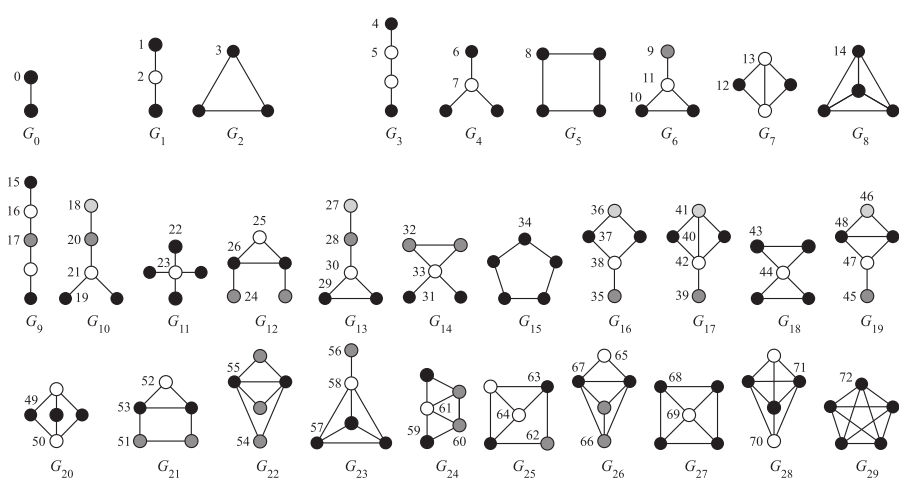
\includegraphics[scale=0.4]{./graphlets.png}
\caption{گرافلت‌های دو تا پنج رأسی. رئوس همرنگ روی هر گرافلت، یک اوربیت را نمایش می‌دهند. شماره هر اوربیت روی یکی از رئوسش مشخص شده‌است.}
\label{fig:graphlets}
\end{figure}

\subsection{الگوریتم ترکیبیاتی شمارش اوربیت‌ها}
فرض کنید $x$ هر رأس از گراف $G$ باشد. مسئله، محاسبه تعداد دفعاتی است که $x$  روی اوربیت $O_i$ از گرافلت‌های القایی گراف $G$ قرار گرفته است. این عدد را با $o_i$ نمایش می‌دهیم. الگوریتم بر اساس دستگاهی از معادل خطی کار می‌کند که تعداد اوربیت‌های مختلف، $o_i$ ها، را به هم مربوط می‌کند. از آنجایی که رتبه این دستگاه یکی کمتر از تعداد انواع اوربیت‌ها خواهد بود می‌توان با شمارش تنها یکی از آن‌ها، تعداد مابقی را بدست آورد. در ادامه، نحوه ساخت و حل این دستگاه برای هر رأس را شرح داده و سپس روش محاسبه تعداد گرافلت‌های گراف از روی تعداد اوربیت رئوس را توضیح می‌دهیم.

\subsubsection{شمارش اوربیت‌های چهار رأسی}
%سمت راست معادلاتی که دستگاه را تشکیل می‌دهد شامل عباراتی است که از گراف $G$ محاسبه می‌شود.
فرض کنید $c(u,v) = |N(u) \cap N(v)|$ تعداد همسایه‌های مشترک دو رأس $u$ و $v$ باشد. همینطور $p(u,v)$ تعداد مسیرهای سه رأسی باشد که از رأس $u$ آغاز می‌شود، به رأس $v$ می‌رود و در رأسی مثل $t$ که به $u$ متصل نیست، پایان می‌یابد. این عدد به راحتی قابل محاسبه است: 
$p(u,v) = deg(v) -1 -c(u,v)$.

اگر رأس $x$ روی یک گرافلت $k$-رأسی مثل $G_i$ قرار گرفته باشد، حتماً روی یک گرافلت $(k-1)$-رأسی مثل $G_j$ هم قرار گرفته است، کافی است دورترین رأس از $x$ را از گراف $G_i$ حذف کنیم. زیرگرافی که از باقی رئوس بوجود می‌آید همبند است (در غیر این صورت، رأسی که جزء مؤلفه همبندی نیست دورترین رأس از $x$ بوده است) بنابراین با یکی از گرافلت‌های $(k-1)$-رأسی مثل $G_j$ یکریخت است.

عکس این مطلب نیز صحیح است: هر گرافلت چهار رأسی را می‌توان با افزودن یک رأس به یکی از گرافلت‌های سه رأسی ساخت. جهت یافتن رابطه تعداد اوربیت‌های گرافلت‌های چهار رأسی برای رأس $x$، تمام اوربیت‌های سه‌رأسی که $x$ روی آن‌ها قرار گرفته است را می‌یابیم و سپس امکان گسترش آن‌ها به گرافلت‌های چهار رأسی را بررسی می‌کنیم.

\begin{figure}[ht]
\centering
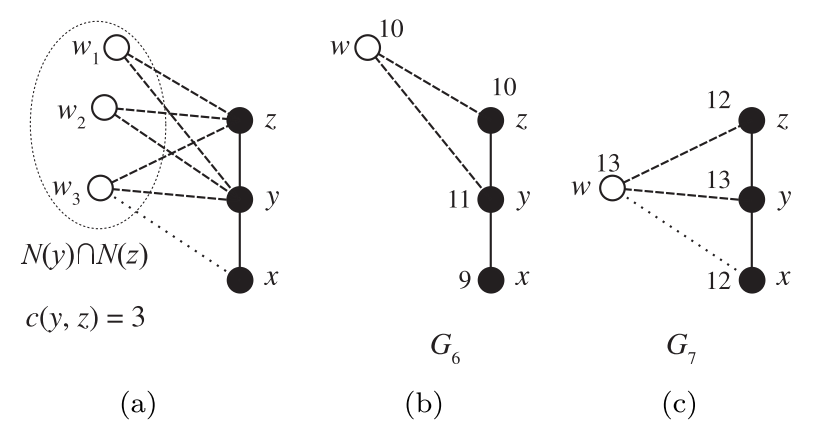
\includegraphics[scale=0.3]{./4-node-graphlet-1.png}
\caption{رابطه بین اوربیت‌های $O_9$ و $O_{12}$.}
\label{fig:o9-o12-relation}
\end{figure}

به عنوان مثال، همانطور که در شکل \ارجا{fig:o9-o12-relation} می‌بینید رئوس $x$،$y$ و $z$ گرافلت $G_1$ را القا می‌کنند که یک مسیر به طول دو است. این گرافلت، توسط $w$ و یال‌های $(w,y)$ و $(w,z)$ به یک گرافلت چهار رأسی تبدیل می‌شود. تعداد رأس‌های ممکن مثل $w$ برابر است با $c(y,z)$. در شکل $c(y,z) = 3$ تا از این رئوس وجود دارد که با $w_1$ ، $w_2$ و $w_3$ نشان داده شده‌اند. یال $(x,w)$ ممکن است در گراف $G$ وجود داشته باشد (مثلاً برای $w_3$ این حالت در نظر گرفته شده) یا ممکن است وجود نداشته باشد (رئوس $w_1$ و $w_2$ اینگونه‌اند). بدون این یال، رئوس $x$ ، $y$ ، $z$ و $w$ گرافلت $G_6$ را تشکیل می‌دهند که $x$ روی اوربیت $O_9$ قرار گرفته است. وجود این یال باعث می‌شود که رئوس مذکور، گرافلت $G_7$ را بسازند که در آن $x$ روی اوربیت $O_{12}$ قرار گرفته‌است. از آنجایی که تمام $c(y,z)$ رأس در $N(y) \cap N(z)$ باید یا در $G_7$ یا در $G_6$ باشند که متقابلاً باعث می‌شود $x$ در $O_9$ یا $O_{12}$ قرار گیرد، پس برای سه‌تایی $x$، $y$ و $z$ خواهیم داشت: $o_9 + o_{12} = c(y,z)$.

حال برای تمام مسیرهای به طول دو که از $x$ شروع می‌شوند، این عدد را جمع می‌زنیم. البته باید دقت داشت که در جمع، تقارن‌ها در نظر گرفته‌شوند: هر گرافلت $G_6$  در گراف $G$ ، با تعویض جای $z$ و $w$ دوبار شمره می‌شود. این اتفاق با تعویض $y$‌ و $w$ برای $G_7$ هم رخ می‌دهد. با این حساب می‌توانیم معادله زیر را تشکیل دهیم:
\begin{equation*}
2o_9+2o_{12} = \sum_{\substack{y,z: x,z\in N(y)\\G[\{x,y,z\}] \simeq G_1 }}c(y,z),
\end{equation*}
که در آن $G[\{x,y,z\}]$ زیرگراف القایی از $G$ است که توسط سه رأس $x$ ، $y$ و $z$ ساخته می‌شود.

\begin{figure}[b]
\centering
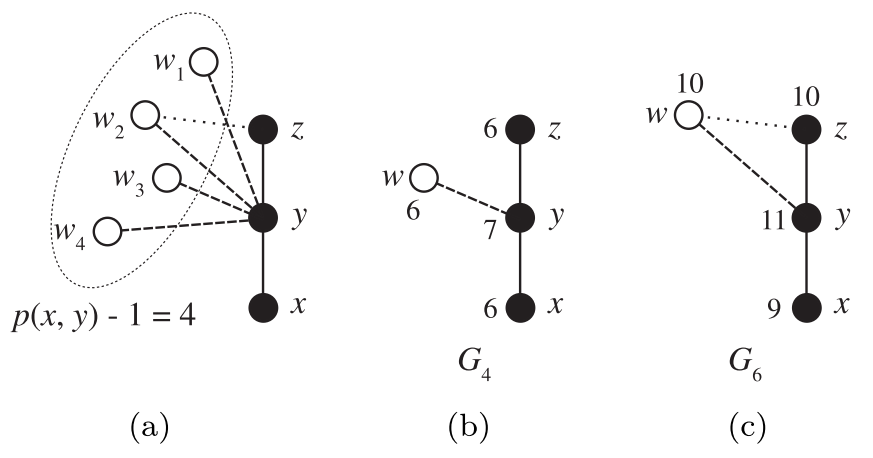
\includegraphics[scale=0.3]{./4-node-graphlet-2.png}
\caption{رابطه بین اوربیت‌های $O_6$ و $O_9$.}
\label{fig:o6-o9-relation}
\end{figure}

برای مثالی دیگر، رابطه بین اوربیت‌های $O_6$ و $O_9$ را بررسی می‌کنیم (شکل \ارجا{fig:o6-o9-relation}). برای اینکار یک مسیر به طول دو از رئوس $x$ ، $y$ و $z$ را توسط یک مسیر دیگر که از $x$ و $y$ شروع می‌شود، گسترش می‌دهیم؛ قبلاً تعداد این مسیرها را با $p(x,y)$ نمادگذاری کردیم. بسته به اینکه رأس جدید ($w$) با $z$ همسایه باشد یا نه، با یک گرافلت $G_6$ یا $G_4$ روبرو هستیم. با احتساب تقارن، و همچنین حذف حالتی که در آن $w=z$ ، خواهیم داشت:
\begin{equation*}
2o_6+2o_9 = \sum_{\substack{y,z: x,z\in N(y)\\G[\{x,y,z\}] \simeq G_1 }}(p(x,y) - 1).
\end{equation*}

از آنجایی که تنها دو گرافلت سه رأسی وجود دارد و حالت‌های گسترش نیز محدود‌اند، می‌توان تمام گسترش‌های ممکن را در نظر گرفت و از آن‌ها یک دستگاه با ده معادله مستقل خطی و یازده متغیر (متناظر با یازده اوربیت گرافلت‌های چهار رأسی) استخراج کرد. در ضمیمه \ارجا{appendix:combinatorial-counting} این معادلات را آورده‌ایم.

عبارات موجود در سمت راست این معادلات، تنها وابسته به گراف $G$ هستند و باید برای هر رأس $x$ محاسبه شوند. برای افزایش سرعت اجرا، برای هر دو رأس $u$ و $v$ مقادیر $c(u,v)$ و $p(u,v)$ را از قبل محاسبه می‌کنیم. البته کافی است این مقادیر را تنها برای رئوس مجاور و نه همه رئوس، بدست آورد زیرا طبق تعریف، $p(u,v)$ فقط برای دو رأس مجاور تعریف می‌شود و همچنین در تمام معادلات به غیر از معادله آخر، $c(u,v)$ تنها برای رئوسی که همسایه هستند مورد نیاز است. بنابراین با اختصاص $O(m)$ فضا، این مقادیر را محاسبه می‌کنیم. برای معادله آخر، کافی است تعداد مسیر‌های به طول دو که از رأس $x$ شروع می‌شوند و به رأس $y$ خاتمه می‌یابند را بشماریم. این کار نیاز به $O(n)$ فضا دارد. چون تعداد اوربیت‌ها را برای هر رأس جداگانه شمارش می‌کنیم، می‌توان از این فضا مجدداً استفاده نمود. با این وصف، مقادیر سمت راست معادله در زمان ثابت و میزان حافظه $O(m+n)$ محاسبه می‌شوند.

همانطور که ذکر شد، برای یافتن مقادیر متغیرها، باید یکی از اوربیت‌ها را شمارش کنیم. اوربیت ۱۴ یا گرافلت چهار رأسی کامل برای این منظور مناسب است زیرا احتمال وقوع آن در یک گراف تُنُک کمتر از مابقی گرافلت‌هاست. در ادامه الگوریتم شمارش این گرافلت را توضیح می‌دهیم.

ساده‌ترین راه برای شمارش تعداد گرافلت‌های $G_8$ که $x_1$ روی آن‌ها قرار دارد، یک الگوریتم مرحله‌ای با شروع از همین رأس است بطوری که در هر مرحله، رأس $x_i$ را که در مجاورت رأس اضافه شده در مرحله قبل یعنی $x_{i-1}$ قرار دارد، به مجموعه رئوس اضافه می‌کنیم اگر این رأس با تمام رئوس اضافه شده قبلی مجاور باشد. پس وقتی می‌خواهیم یکی از همسایه‌های $x_3$ را به عنوان $x_4$ اضافه کنیم، باید بررسی کنیم که آیا این رأس با $x_1$ و $x_2$ مجاور است یا خیر. با فرض اینکه با یک گراف تنک سر و کار داریم، این امر به ندرت اتفاق می‌افتد.

یک راه بهتر این است که ابتدا همسایه‌های مشترک $x_1$ و $x_2$ را در نظر بگیریم. اینکار در $O(d)$ امکان‌پذیر است. سپس یک دوتای مثل $(x_3,x_4)$ را از این مجموعه انتخاب می‌کنیم و بررسی می‌کنیم که رئوس این دوتایی، مجاور باشند. کاندید‌هایی که از این طریق انتخاب می‌شوند، برخلاف الگوریتم قبل، تنها باید در یک شرط صدق کنند.

برای جلوگیری از شمارش دوباره یک گرافلت، ترتیب قراردادی $x_2 < x_3 < x_4$ را در نظر می‌گیریم. اگرچه هر دو الگوریتم از نظر تئوری، پیچیدگی یکسان و برابر$O(d^3)$ دارند ولی در عمل برای گراف‌های تنک، الگوریتم دوم بسیار سریعتر است.

این روش را می‌توان برای شمارش گرافلت‌های کامل پنج رأسی و بیشتر هم بکار برد. در هر مرحله، لیست $C_i$ از رئوس کاندید برای $x_i$ را نگهداری می‌کنیم بطوری که این رئوس با تمام رئوس قبل مجاور باشند. یکی از این کاندیدها را به عنوان $x_i$ انتخاب کرده و لیست $C_{i+1} = C_i\cap N(x_i)$ را تشکیل می‌دهیم و اینکار را تا جایی که به تعداد رئوس مورد نظر برسیم ادامه می‌دهیم. برای شمارش تمام گرافلت‌های کامل $k$-رأسی روی رأس $x$، این الگوریتم در زمان $O(d^{k-1})$ قابل اجراست.

حال که تعداد اوربیت $O_{14}$ را داریم، می‌توانیم در زمان ثابت، معادلات را حل کرده و تعداد اوربیت‌های هر رأس را بدست آوریم. بنابراین کل زمان اجرا برای محاسبه تعداد اوربیت‌های تمام رئوس برابر است با $O(m.d+T_4)$ که $O(T_4) = O(d^3)$ زمان مورد نیاز برای شمارش گرافلت‌های کامل روی چهار رأس است.

\subsubsection{شمارش اوربیت‌های پنج رأسی}
برای شمارش اوربیت‌های چهار رأسی، تمام حالت‌های ممکن جهت گسترش یک گرافلت سه رأسی به گرافلت چهار رأسی را در نظر گرفتیم. اینکار برای گذر از چهار رأس به پنج رأس ممکن نیست زیرا تعداد بسیار زیادی معادله بوجود می‌آید که مستقل نیستند. پس راه دیگری را پیش می‌گیریم: برای هر اوربیت، فرض می‌کنیم رأس مورد نظر یعنی $x$ روی این اوربیت قرار گرفته است. یک رأس مثل $y$ از گرافلت متناظر انتخاب می‌کنیم و بررسی می‌کنیم که با اضافه کردن یال بین $y$ و دیگر رئوس این گرافلت، اوربیت $x$ چه تغییری می‌کند.

\begin{figure}[t]
\centering
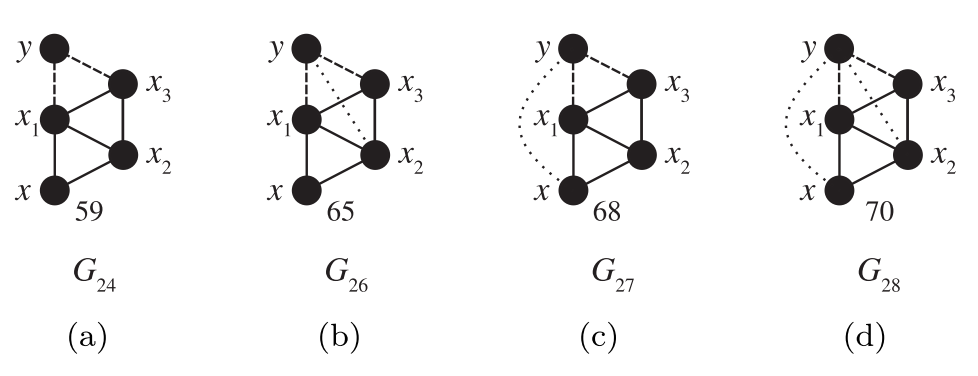
\includegraphics[scale=0.3]{./o59-orbit-relation.png}
\caption{شمارش اوربیت ۵۹. اضافه کردن یال بین رأس $y$ و دیگر رئوس باعث قرار گرفتن $x$ در اوربیت‌های مختلف می‌شود.}
\label{fig:o59-orbit-relation}
\end{figure}

در شکل \ارجا{fig:o59-orbit-relation}، رأس $x$ در اوربیت $O_{59}$ از گرافلت $G_{24}$ قرار گرفته و رأس $y$ مشخص گردیده‌است. باقی رئوس با برچسب‌گذاری $x_1$، $x_2$ و $x_3$ مشخص شده‌اند. توجه کنید که حذف $y$ باعث کاهش $G_{24}$ به $G_7$ می‌شود که در این حالت $x$ روی اوربیت $O_{12}$ قرار می‌گیرد.

حال فرض کنید که در حال شمارش اوربیت‌های رأس $x$ هستیم و با زیرگراف القایی $H \simeq G_{7}$ روبرو می‌شویم که $x$ روی اوربیت $O_{12}$ قرار گرفته‌است. رئوس دیگر این زیرگراف را مانند شکل با $x_1$، $x_2$ و $x_3$ برچسب‌گذاری می‌کنیم. در گراف $G$، به تعداد $c(x_1,x_3)$ برای دو رأس $x_1$ و $x_3$ همسایه مشترک وجود دارد. ممکن است بعضی از این رئوس با $x$ یا $x_2$ و یا هر دوی آن‌ها نیز همسایه باشند. شکل \ارجا{fig:o59-orbit-relation} تمام چهار حالت ممکن را نمایش می‌دهد که گرافلت‌های $G_{24}$، $G_{26}$، $G_{27}$ و $G_{28}$ را بوجود می‌آورند و $x$ به ترتیب در اوربیت‌های ۵۹، ۶۵، ۶۸ و ۷۰ قرار می‌گیرد. بنابراین رابطه $o^\prime_{59}+ o^\prime_{65}+o^\prime_{68}+o^\prime_{70} = c(x_1,x_3)$ بدست می‌آید که در آن $o^\prime_i$ تعداد اوربیت‌های $x$ با توجه به زیرگراف $H$ است. برای بدست آوردن ارتباط $o_{59}$ ،  $o_{65}$ ،  $o_{68}$ و  $o_{70}$ باید این عبارت را روی تمام زیرگراف‌های القایی $G_7$ که $x$ روی اوربیت ۱۲ قرار می‌گیرد، جمع کنیم. با احتساب تقارن‌هایی که با تغییر برچسب‌گذاری‌ بوجود می‌آید خواهیم داشت:
\begin{equation*}
o_{59}+4o_{65}+2o_{68}+6o_{70} = \sum_{\substack{x_1,x_2,x_3:\\x_1 < x_2\wedge x_3 \notin N(x),\\G[\{x,x_1,x_2,x_3\}]\simeq G_7}}{c(x_1,x_3)+c(x_2,x_3)}
\end{equation*}
شرط $x_1 < x_2$ تحت یک برچسب‌گذاری دلخواه روی رئوس، برای جلوگیری از شمارش دوباره گرافلت $G_7$ ضروری است. دو شرط بعد، موقعیت $x$ در اوربیت ۱۲ را بررسی می‌کنند. عبارت $c(x_2,x_3)$ حالتی را در نظر می‌گیرد که نقش $x_1$ و $x_2$ جابجا شده‌باشد.

با استفاده از این تکنیک روی دیگر اوربیت‌ها به غیر از $O_{72}$،
 ۵۷ معادله مستقل خطی برای ۵۸ اوربیت خواهیم داشت. مانند شمارش اوربیت‌های چهار رأسی، در اینجا نیز $O_{72}$ را که گرافلت کامل پنج رأسی است، بطور کامل شمارش می‌کنیم. روش ساخت معادلات، مستقل خطی بودن آن‌ها را تضمین می‌کند: هر معادله با در نظر گرفتن یک اوربیت تشکیل می‌شود (مثل اوربیت $O_{59}$ در مثال بالا) و دیگر اوربیت‌هایی که در معادله ظاهر می‌شوند مربوط به گرافلت‌هایی هستند که تعداد یال‌های بیشتری دارند (یال‌هایی که به صورت نقطه‌چین بین $y$ و دیگر رئوس در شکل \ارجا{fig:o59-orbit-relation} نمایش داده شده‌اند).
 
در هنگام ساخت معادلات، رأس $y$ را بگونه‌ای انتخاب می‌کنیم که محاسبه عبارات سمت راست معادله، بهینه باشد. یعنی عبارات سمت راست تنها شامل درجه رئوس، تعداد همسایه‌های مشترک جفت رئوس مجاور، $c(u,v)$، و یا تعداد سه‌تایی‌های متصل، $c(u,v,t)$، باشد.

برای اینکار، $y$ باید طوری انتخاب شود که اولاً  باقی رئوس، یک گرافلت چهار رأسی را تشکیل بدهند. یعنی حذف $y$ گرافلت را به دو قسمت تقسیم نکند. دوماً رأس $y$ باید حداکثر سه یال به رئوس گرافلت مورد نظر داشته باشد. اینکار از شمارش تعداد چهارتایی‌های متصل ($c(u,v,t,w)$) جلوگیری می‌کند. و در نهایت اگر $y$ سه همسایه داشته باشد، باید این سه همسایه، متصل باشند. رأسی که در این شروط صدق کند برای همه اوربیت‌ها به غیر از اوربیت $O_{72}$ وجود دارد.

محاسبه مقادیر $c(u,v,t)$‌ برای تمام سه‌تایی‌های متصل، در زمان $O(e.d^2)$ و ذخیره در فضای $O(e.d)$، قابل انجام است. همچنین محاسبه عبارات سمت راست، نیاز به شمارش تمام گرافلت‌های چهار رأسی دارد که در زمان $O(e.d^2)$ قابل انجام است. بنابراین شمارش تمام اوربیت‌ها برای تمام رئوس گراف $G$ در زمان $O(e.d^2 + T_5)$ و فضای $O(e.d)$ انجام می‌شود که در آن $O(T_5)$ زمان لازم برای شمارش تمام گرافلت‌های کامل پنج رأسی ($G_{29}$) است. نتیجه می‌شود که کران بالای زمان اجرای این الگوریتم برابر $O(n.d^4)$ است. البته سهم $O(T_5)$ در زمان اجرا معمولاً به حدی کم است که قابل چشم‌پوشی است زیرا گرافلت پنج رأسی کامل به ندرت در گراف‌ها به چشم می‌خورد.

\subsection{تبدیل تعداد اوربیت‌ها به تعداد گرافلت‌ها}
تا اینجا برای هر رأس $x$ از گراف $G$، یک بردار با ۷۳ مؤلفه معادل ۷۳ اوربیت ساخته‌ایم که مؤلفه $i$ از این بردار، برابر $o_i$ محاسبه شده برای این رأس است. این عدد نشان می‌دهد که $x$ روی چند اوربیت از نوع $O_i$ قرار دارد. همچنین می‌توان به $x$، برداری ۲۹ تایی از تعداد گرافلت‌هایی که این رأس روی آن‌هاست، نسبت داد. هر مؤلفه $i$ از این بردار، نشان می‌دهد که $x$ روی چند گرافلت از نوع $G_i$ قرار دارد. برای محاسبه این بردار، کافی است $o_i$ هایی را که متعلق به یک گرافلت هستند، با هم جمع کنیم.

حال می‌خواهیم تعداد کل تکرار هر گرافلت‌ در گراف $G$ را بدست آوریم. نتیجه، یک بردار ۲۹ تایی مثل $C_G$ خواهد بود که هر مؤلفه $i$ از آن، تعداد تکرار گرافلت $G_i$ در گراف $G$ را نشان می‌دهد. هر نمونه از گرافلت $G_i$ در گراف $G$، یکبار توسط هر رأسش دیده می‌شود. در نتیجه، بردارهای گرافلت تمام رئوس گراف را با هم جمع کرده و هر مؤلفه را بر اندازه گرافلت متناظرش تقسیم می‌کنیم. بردار حاصل، $C_G$ خواهد بود.

\section{گرافلت کرنل گاوسی}
فرض کنید برای دو گراف $G$ و $G^\prime$ ، بردار شمارش گرافلت‌ها، $C_G$ و $C_{G^\prime}$ را در اختیار داریم. حال باید این دو بردار را با یکدیگر مقایسه کرده و فاصله آن‌ها را تعیین کنیم. برای کاهش تأثیر اندازه گراف‌ بر مقایسه و همچنین جلوگیری از تأثیر فراوانی زیاد یک گرافلت بر کل مقایسه، بردارها را به صورت
\begin{equation}
\label{eq:feature-vector}
\hat{C}_G = (-\log(\dfrac{C_G(0)}{\sum _{i=0}^{29} C_G(i)}),...,-\log(\dfrac{C_G(29)}{\sum _{i=0}^{29} C_G(i)}))
\end{equation}
نرمال می‌کنیم و از تابع کرنل گاوسی برای مقایسه این بردارها بهره می‌بریم. بنابراین گرافلت کرنل گاوسی $k$ را به صورت
\begin{equation}
\label{eqn:kernelfunction}
k(G,G') = exp(-\gamma\parallel \hat{C}_G - \hat{C}_{G'}\parallel^2)
\end{equation}
تعریف می‌کنیم که در آن $\gamma = \dfrac{1}{2\sigma^2}$ است.

\section{عملکرد گرافلت کرنل گاوسی}
در این بخش، عملکرد گرافلت کرنل گاوسی را در تشخیص و جداسازی مدل‌های گراف تصادفی از یکدیگر، می‌سنجیم. گراف تصادفی، گرافی است که توسط یک روند تصادفی ساخته می‌شود. یک مدل‌ گراف تصادفی، در واقع تعریف یک تابع احتمال خاص برای انتخاب گراف‌ها از گردایه‌ی تمام گراف‌های تصادفیِ ممکن است. این توزیع بگونه‌ای تعریف می‌شود که گراف‌های انتخابی دارای یک مشخصه مشترک باشند. مدل‌هایی که در ادامه به آن‌ها نیاز خواهیم داشت به شرح زیراند:

\paragraph{مدل تصادفی اردوش و رنی (ER)}
اردوش\پانوشت{\متن‌لاتین{Erdős}} و رنی\پانوشت{\متن‌لاتین{Rényi}} در سال ۱۹۵۹ مدلی برای گراف‌های تصادفی ارائه دادند\جستار{Erdos_1959} که اکنون به مدل \متن‌لاتین{ER} معروف است. گراف تصادفی اردوش-رنی $G(n,p)$، یک گراف با $n$ رأس است که در آن، یال‌ها به صورت مستقل و به احتمال $p$ از بین تمام یال‌های ممکن انتخاب شده‌اند. گرافی که با این روند تولید شود دارای توزیع درجه دوجمله‌ای است. برای $n$ های بزرگ، توزیع درجه، پواسون خواهد بود.

\paragraph{مدل تصادفی واتس و استروگاتس (WS)}
این مدل در سال ۱۹۹۸ توسط واتس\پانوشت{\متن‌لاتین{Duncan J. Watts}} و استروگاتس\پانوشت{\متن‌لاتین{Steven Strogatz}} معرفی شد\جستار{Watts_1998} و اولین مدلی است که خاصیت جهان کوچک\پانوشت{\متن‌لاتین{Small-World}} را شبیه سازی می‌کند. این خاصیت بیان می‌کند که هر دو فرد در جهان با چند واسطه به یکدیگر متصل می‌شوند و تعداد این واسطه‌ها زیاد نیست (معمولاً بین ۳ تا ۶ واسطه). یک گراف تصادفی واتس و استروگاتس روی $N$ رأس، با میانگین درجه $K$ و پارامتر $\beta$ (
$0\leq \beta \leq 1$ و $N \geq K \geq ln(N) \geq 1$
) به صورت زیر ساخته می‌شود:
\begin{enumerate}
\فقره گرافی با $N$ رأس و هر رأس با $K$ همسایه، $K/2$ در سمت راست و $K/2$ در سمت چپ، در نظر گرفته می‌شود.
\فقره اگر رئوس را با برچسب‌گذاری $n_0,\ldots,n_N-1$ مشخص کنیم، برای هر رأس، هر یال $(n_i,n_j)$ که $i < j$ به احتمال $\beta$ بازنشانی\پانوشت{\متن‌لاتین{rewire}} می‌شود. در اینجا، بازنشانی یعنی تعویض یال $(n_i,n_j)$ با یال $(n_i,n_k)$ که $n_k$ به احتمال یکنواخت از بین دیگر رئوس انتخاب می‌شود به شرطی که گراف، ساده باقی بماند.
\end{enumerate}

\paragraph{مدل تصادفی باراباشی و آلبرت (BA)}
مدل تصادفی باراباشی\پانوشت{\متن‌لاتین{Barabasi}}-آلبرت\پانوشت{\متن‌لاتین{Albert}} در سال ۱۹۹۹ برای مدل‌سازی خاصیت \متن‌لاتین{scale-free} در شبکه‌های واقعی (مثل شبکه وب و یا خطوط انتقال برق)، طراحی شد\جستار{Barabasi_1999}. این خاصیت بیان می‌کند که اولاً شبکه‌ها در حال رشد کردن هستند یعنی به تعداد رئوس آن‌ها اضافه می‌شود، و ثانیاً احتمال بوجود آمدن یال بین رئوس جدید و رئوسی که بیشترین درجه را دارند، بیشتر است. این خاصیت در واقع اشاره‌ای به \خمیده{اثر متیو}\پانوشت{\متن‌لاتین{Matthew}} است که بیان می‌کند «پولدار، پولدارتر می‌شود»\جستار{Merton_1968}. برای تولید گراف با این خاصیت، یک گراف همبند با $n$ رأس در نظر گرفته می‌شود. رئوس جدید، یکی یکی به گراف افزوده می‌شوند. هر رأس جدید می‌تواند به $n$ رأس قبل به احتمالی بر حسب درجه رئوس، متصل شود. احتمال اینکه رأس جدید به رأس $n_i$ متصل شود برابر است با
$\dfrac{k_i}{\sum_jk_j}$ 
که $k_i$ درجه رأس $n_i$ و جمع، روی کل رئوس گراف تا لحظه اضافه کردن $n_i$ است. گرافی که با این روند ساخته شود، دارای توزیع درجه \خمیده{\متن‌لاتین{power law}}  با پارامتر $\lambda = 3$ است. این توزیع به شکل $P(k) \sim k^{-\lambda}$ تعریف می‌شود.

\paragraph{مدل تصادفی هندسی (GEO)}
مدل گراف تصادفی هندسی برای مدل‌سازی و تحلیل شبکه‌های سنسور بی‌سیم\جستار{Bettstetter_2002} و همچنین شبکه‌های تعاملات پروتئینی\جستار{Przulj_2004} مورد استفاده قرار گرفته است. در این مدل، 
برای ساخت یک گراف تصادفی هندسی با $n$ رأس و به شعاع $r$، $n$ نقطه متناظر با رئوس در فضای $\R^d$ به طول واحد به صورت تصادفی و به احتمال یکنواخت قرار داده می‌شوند. بین رئوس متناظر با نقاطی که فاصله اقلیدسی آن‌ها کمتر از $r$ باشد، یال قرار داده می‌شود.

\paragraph{مدل ترتیبی ساخت گراف تصادفی (CM)}
هدف از ارائه این مدل، ساخت گراف از روی دنباله درجه دلخواه، و در نتیجه، توزیع درجه دلخواه بوده‌است\جستار{Molloy_1995}. در این مدل، برای هر دنباله درجه قابل قبول (یعنی جمع اعداد دنباله، عددی زوج باشد)، از گردایه‌ی گراف‌ها با آن توزیع درجه، یک گراف به صورت تصادفی انتخاب می‌شود. البته باید توجه داشت که گراف‌های حاصل الزاماً ساده نیستند. برای تبدیل گراف به یک گراف ساده، طوقه‌ها و یال‌های چندگانه از گراف حذف می‌شوند. اینکار باعث تغییر در دنباله درجه می‌شود که البته در گراف‌های بزرگ، این تغییر قابل چشم‌پوشی است. در این مدل، متناسب با دنباله درجه داده شده مثل $\vec{k}$، $n$ رأس در نظر گرفته می‌شود. به هر رأس $n_i$ متناسب با درجه در نظر گرفته شده برای آن، $k_i$ نیم یال نسبت داده می‌شود. نیم‌یال‌ها به صورت تصادفی به یکدیگر متصل می‌شوند. نتیجه یک گراف با توزیع درجه داده‌ شده خواهد بود.

\subsection{داده‌‌ها}
از مدل‌های تصادفی معرفی شده، گراف‌هایی با اندازه ۱۰ تا ۱۰۰۰ رأس تولید شد. جدول \ارجا{tab:random-graph-datasets-statistics} پارامترهای انتخابی برای هر مدل و تعداد گراف‌های تولید شده را مشخص کرده‌است. ذکر این نکته ضروری است که تضمینی برای همبندی گراف‌های تولید شده برای بعضی مدل‌ها وجود ندارد. به همین دلیل، پس از تولید گراف‌ها، بزرگترین مؤلفه همبندی هر کدام استخراج و به عنوان گراف نهایی مورد استفاده قرار گرفته‌است. در بعضی مواقع، دو مؤلفه همبندی اندازه یکسان داشته‌اند که در این صورت، یکی از آن‌ها به صورت تصادفی حذف شده‌است. لذا تعداد گراف‌های نهایی برای مدل‌های مختلف، متفاوت است. همچنین توجه شود که از مدل ترتیبی ساخت گراف تصادفی برای تولید گراف‌هایی با توزیع درجه \متن‌لاتین{power law} در توان‌های مختلف استفاده شده‌است. برای این مدل‌ها، ستون پارامتر، توان تابع توزیع را مشخص می‌کند.

\begin{table}[ht]
\centering
\begin{tabular}{| c | c | c | c | c | c | c |}
    \hline
    نام & مدل & تعداد گراف‌ها & پارامتر‌ها & متوسط تعداد رئوس & متوسط تعداد یال‌ها \\[5pt] \hline
\lr{ER} & ER & ۹۵۴ & $p = 0.05$ & ۵۲۱ & ۸۷۳۳ \\
\lr{WS} & WS & ۹۹۳ & $k = 5,p = 0.5$ & ۵۰۶ & ۱۵۱۶ \\
\lr{GEO} & GEO & ۷۳۹ & $r = 0.04$ & ۴۶۴ & ۱۲۱۳ \\
\lr{PW1} & CM & ۹۸۷ & $\lambda = 2.50$ & ۵۰۹ & ۷۱۲ \\
\lr{PW2} & CM & ۹۸۰ & $\lambda = 2.75$ & ۵۰۴ & ۶۰۶ \\
\lr{PW3} & CM & ۹۹۴ & $\lambda = 3.00$ & ۵۰۴ & ۵۵۵ \\
\lr{PW4} & CM & ۹۶۴ & $\lambda = 3.25$ & ۴۸۷ & ۵۰۹ \\ \hline
\end{tabular}
\caption{
گراف‌های تولید شده با استفاده از مدل‌های تصادفی گراف. ER نمایش دهنده مدل تصادفی اردوش-رنی، WS نمایش دهنده مدل تصادفی واتس-استروگاتس، GEO نمایش دهنده مدل تصادفی هندسی و \lr{PW1} تا \lr{PW4} نمایش‌دهنده مدل‌ تصادفی ترتیبی هستند. لازم به ذکر است که \lr{PW3} همان مدل باراباشی-آلبرت می‌باشد.
}
\label{tab:random-graph-datasets-statistics}
\end{table}

\subsection{جداسازی گراف‌های scale-free از یکدیگر}
با تغییر در پارامتر $\lambda$، ساختار گراف‌های scale-free و بسیاری از مشخصه‌های آن‌ها از جمله طول کوتاهترین مسیر، قطر گراف، تعداد یال‌ها، ضریب خوشه‌بندی و ... تغییر می‌کند. شکل \ارجا{fig:scale-free-distance} شباهت گراف‌های مجموعه‌های \متن‌لاتین{PW2}، \متن‌لاتین{PW3} و \متن‌لاتین{PW4} نسبت به گراف‌های مجموعه \متن‌لاتین{PW1} را با استفاده از گرافلت‌کرنل گاوسی (با پارامتر $\gamma = 2$) نشان می‌دهد. در این شکل، محور افقی اندازه گراف و محور عمودی، فاصله گراف‌ها از گراف‌های مرجع (\متن‌لاتین{PW1}) را مشخص می‌کند. هر چه این عدد برای یک گراف به یک نزدیکتر باشد، یعنی این گراف شباهت کمتری به گراف متناظر در \متن‌لاتین{PW1} دارد.

\begin{figure}[t]
\centering
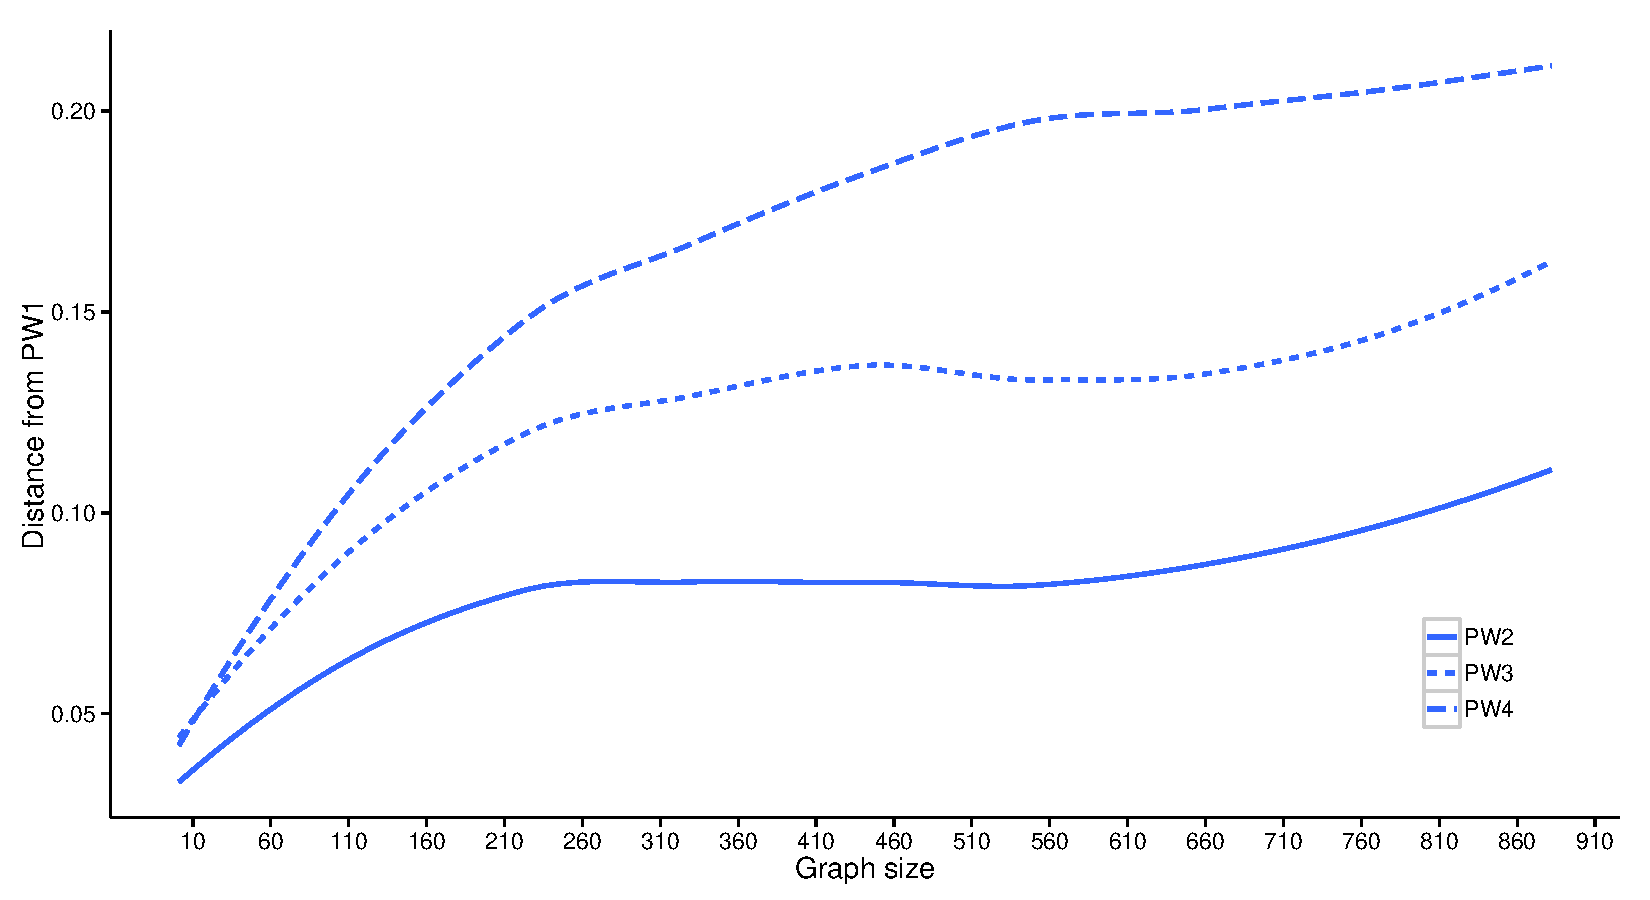
\includegraphics[scale=0.5]{./scale-free-distance.pdf}
\caption{فاصله گراف‌های \lr{PW2} و \lr{PW3} و \lr{PW4} از گراف مرجع \lr{PW1} با استفاده از گرافلت کرنل گاوسی با پارامتر $\gamma = 2$.}
\label{fig:scale-free-distance}
\end{figure}

به نظر می‌رسد که گرافلت کرنل گاوسی می‌تواند بخوبی بین گراف‌های \متن‌لاتین{scale-free} با پارامتر‌های مختلف، تفاوت قائل شود. با استفاده از یک ماشین \متن‌لاتین{C-SVM} میزان دقت کرنل در تفکیک این گراف‌ها اندازه‌گیری شده‌است. نحوه انجام اندازه‌گیری به این شرح است که ابتدا داده‌ها به صورت تصادفی به ۱۰ قسمت تقسیم شده‌اند. از ۹ قسمت برای آموزش ماشین، و از قسمت باقی مانده برای سنج دقت، استفاده شده‌است. به این کار، \متن‌لاتین{10-fold cross validation} گفته می‌شود. پس از میزان کردن پارامتر‌ $C$ برای ماشین و $\gamma$ برای کرنل، و ۱۰ بار تکرار آزمایش، نتایج موجود در جدول \ارجا{tab:svm-scale-free} بدست آمد.

\begin{table}[ht]
\centering
\begin{tabular}{| c | c | c |}
    \hline
مدل‌ها & پارامتر‌های انتخاب & میزان دقت
  \\[5pt] \hline
\lr{PW1} در مقابل \lr{PW2} & $C=10, \gamma = 0.01$ & 81\% \\ \hline
\lr{PW1} در مقابل \lr{PW3} & $C=10, \gamma = 0.01$ & 80\% \\ \hline
\lr{PW1} در مقابل \lr{PW4} & $C=10, \gamma = 0.01$ & 84\% \\ \hline
\end{tabular}
\caption{
دقت کرنل در تفکیک گراف‌های \متن‌لاتین{scale-free} از یکدیگر. برای هر گروه، بهترین پارامتر‌ها توسط $SVM$ انتخاب شده‌است.
}
\label{tab:svm-scale-free}
\end{table}

\subsection{جداسازی گراف‌های تصادفی \lr{GEO}، \lr{BA}، \lr{WS}، \lr{ER}}
شکل \ارجا{fig:random-graph-distance} شباهت گراف‌های تصادفی تولید شده در مدل‌های \متن‌لاتین{ER}، \متن‌لاتین{GEO}، \متن‌لاتین{WS} به گراف‌های \متن‌لاتین{BA} را با استفاده از گرافلت‌کرنل گاوسی (با پارامتر $\gamma = 2$) نشان می‌دهد. همانطور که مشخص است، در اندازه‌های کوچک، شباهت گراف‌ها به یکدیگر بسیار زیاد است. اما با افزایش اندازه گراف‌ها، کرنل می‌تواند تفاوت‌ها را بهتر تشخیص دهد. جدول \ارجا{tab:svm-random-graph}، حاصل انجام آزمایش مشابه بخش قبل، روی این گراف‌هاست. به نظر می‌رسد دقت بالای کرنل در تشخیص گراف‌های \متن‌لاتین{ER} از گراف‌های \متن‌لاتین{BA}، به دلیل تفاوت زیاد در چگالی گراف‌هاست. چگالی یک گراف، نسبت یال‌های گراف به تمام یال‌های ممکن در آن گراف ($\dfrac{n(n-1)}{2}$) است.

\begin{figure}[t]
\centering
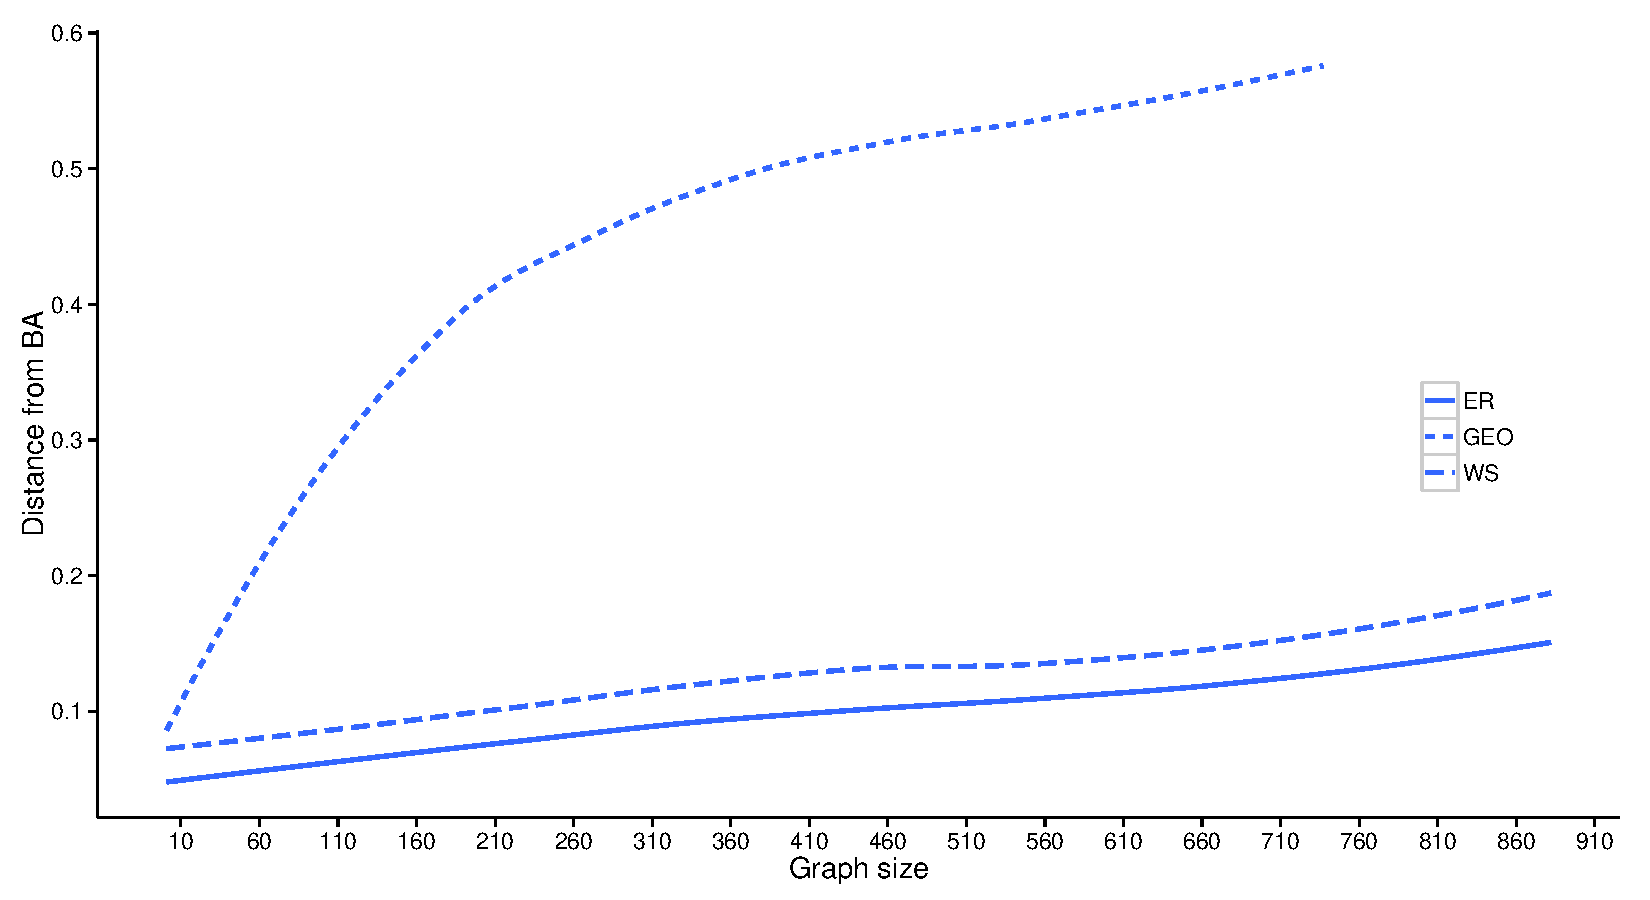
\includegraphics[scale=0.5]{./random-graph-distance.pdf}
\caption{فاصله گراف‌های \lr{ER} و \lr{GEO} و \lr{WS} از گراف‌های مرجع \lr{BA} با استفاده از گرافلت کرنل گاوسی با پارامتر $\gamma = 2$.}
\label{fig:random-graph-distance}
\end{figure}

\begin{table}[ht]
\centering
\begin{tabular}{| c | c | c |}
    \hline
مدل‌ها & پارامتر‌ها & میزان دقت
  \\[5pt] \hline
\lr{BA} در مقابل \lr{ER} & $C=10, \gamma = 10$ & 96\% \\ \hline
\lr{BA} در مقابل \lr{WS} & $C=10, \gamma = 10$ & 82\% \\ \hline
\lr{BA} در مقابل \lr{GEO} & $C=10, \gamma = 10$ & 81\% \\ \hline
\end{tabular}
\caption{
دقت کرنل در تفکیک گراف‌های \متن‌لاتین{scale-free} از یکدیگر. برای هر گروه، بهترین پارامتر‌ها توسط $SVM$ انتخاب شده‌است.
}
\label{tab:svm-random-graph}
\end{table}

\subsection{گرافلت یا اوربیت؟}\label{sec:graphlet-vs-orbit}
شاید به نظر برسد که اوربیت‌ها، اطلاعات دقیقتری از شبکه بدست می‌دهند. چنین تصوری برای تحلیل رئوس گراف درست است. اما آزمایش نشان می‌دهد که برای مقایسه گراف‌ها، استفاده از بردار ۷۳تایی اوربیتیِ گراف، از دقت گرافلت کرنل گاوسی می‌کاهد. جدول \ارجا{tab:graphlet-vs-orbit} دقت گرافلت کرنل گاوسی در تفکیک انواع گراف‌های \متن‌لاتین{scale-free} را با استفاده از بردار گرافلت و بردار اوربیت، نشان می‌دهد. پارامتر‌های انتخاب شده، پارامتر‌هایی است که در آن هر دو کرنل بهترین جواب‌ها را داشتند. 

\begin{table}[h]
\centering
\begin{tabular}{| c | c | c | c |}
    \hline
مدل‌ها & پارامتر‌ها & کرنل گرافلتی & کرنل اوربیتی
  \\[5pt] \hline
\lr{PW1} در مقابل \lr{PW2} & $C=10, \gamma = 0.01$ & 81\% & 70\%\\ \hline
\lr{PW1} در مقابل \lr{PW3} & $C=10, \gamma = 0.01$ & 80\% & 70\%\\ \hline
\lr{PW1} در مقابل \lr{PW4} & $C=10, \gamma = 0.01$ & 84\% & 71\%\\ \hline
\end{tabular}
\caption{
دقت تشخیص گراف‌های تصادفی \متن‌لاتین{PW2}، \متن‌لاتین{PW3} و \متن‌لاتین{PW4} از گراف‌های \متن‌لاتین{PW1} با استفاده از بردار اوربیتی در گرافلت کرنل گاوسی (کرنل گرافلتی) و بردار گرافلتی در گرافلت کرنل گاوسی (کرنل گرافلتی).
}
\label{tab:graphlet-vs-orbit}
\end{table}

\section{جمع‌بندی}
در این فصل، الگوریتم شمارش بهینه گرافلت‌ها را شرح دادیم و گرافلت کرنل گاوسی را بر مبنای بردار گرافلت و تابع کرنل گاوسی، تعریف کردیم. سپس از این کرنل در تشخیص و جداسازی انواع گراف‌های تصادفی استفاده نمودیم. همانطور که از نتایج مشخص است، این کرنل قابلیت خوبی در تشخیص ساختار گراف‌ها دارد. در فصل بعد، از این کرنل روی داده‌های واقعی استفاده کرده و آن‌را با دیگر گراف کرنل‌ها مقایسه می‌کنیم.